\chapter{Introduction}

\section{Nuclear Power}

Towards the second half of the twentieth century, the energy confined within atomic nuclei was first utilised for commercial electrical power. This marked a significant departure from previous forms of commercial energy production, which relied on less energetically lucrative sources such as combustion of coal, oil and gas. Indeed, the closest we had come to utilising nuclear energy commercially was through geothermal power, where the thermal energy is partly due to radiogenic heat from unstable isotopes in the Earth's mantle \cite{gando2011partial} . 
%which relied on the chemical reactions of coal oil and gas
%Combustion is a chemical process, where energy differences between reactants and products are exploited via electron exchange. Nuclear energy however, exploits the energy difference between nuclei. Both rely on the conversion of mass into energy, however, the amount of energy that can be extracted varies by several orders of magnitude
Combustion is a chemical process where energy differences between reactants and products are exploited via electron exchange. Nuclear energy however, exploits the energy difference between nuclei. Both rely on the conversion of mass into energy, however, the amount of energy that can be extracted from the nucleus is several orders of magnitude greater.
%Combustion is a chemical process, and its use in commercial energy production is fundamentally about exploiting the free energy difference when electrons are exchanged between some reactants to produce some products. Nuclear energy, however, is about the direct conversion of mass into energy. The difference between the two is staggering.

Consider methane, with an enthalpy of combustion of −887.2 kJ/mol \cite{thornton1917xv}. This is the equivalent of 9.14 eV per particle. By comparison, the energy release from fission of one uranium-235 nucleus is at least $1.65 \times 10^{8}$ eV, as shown in Figure \ref{figure:fissionenergy}.

\begin{figure}[htp]
\centering
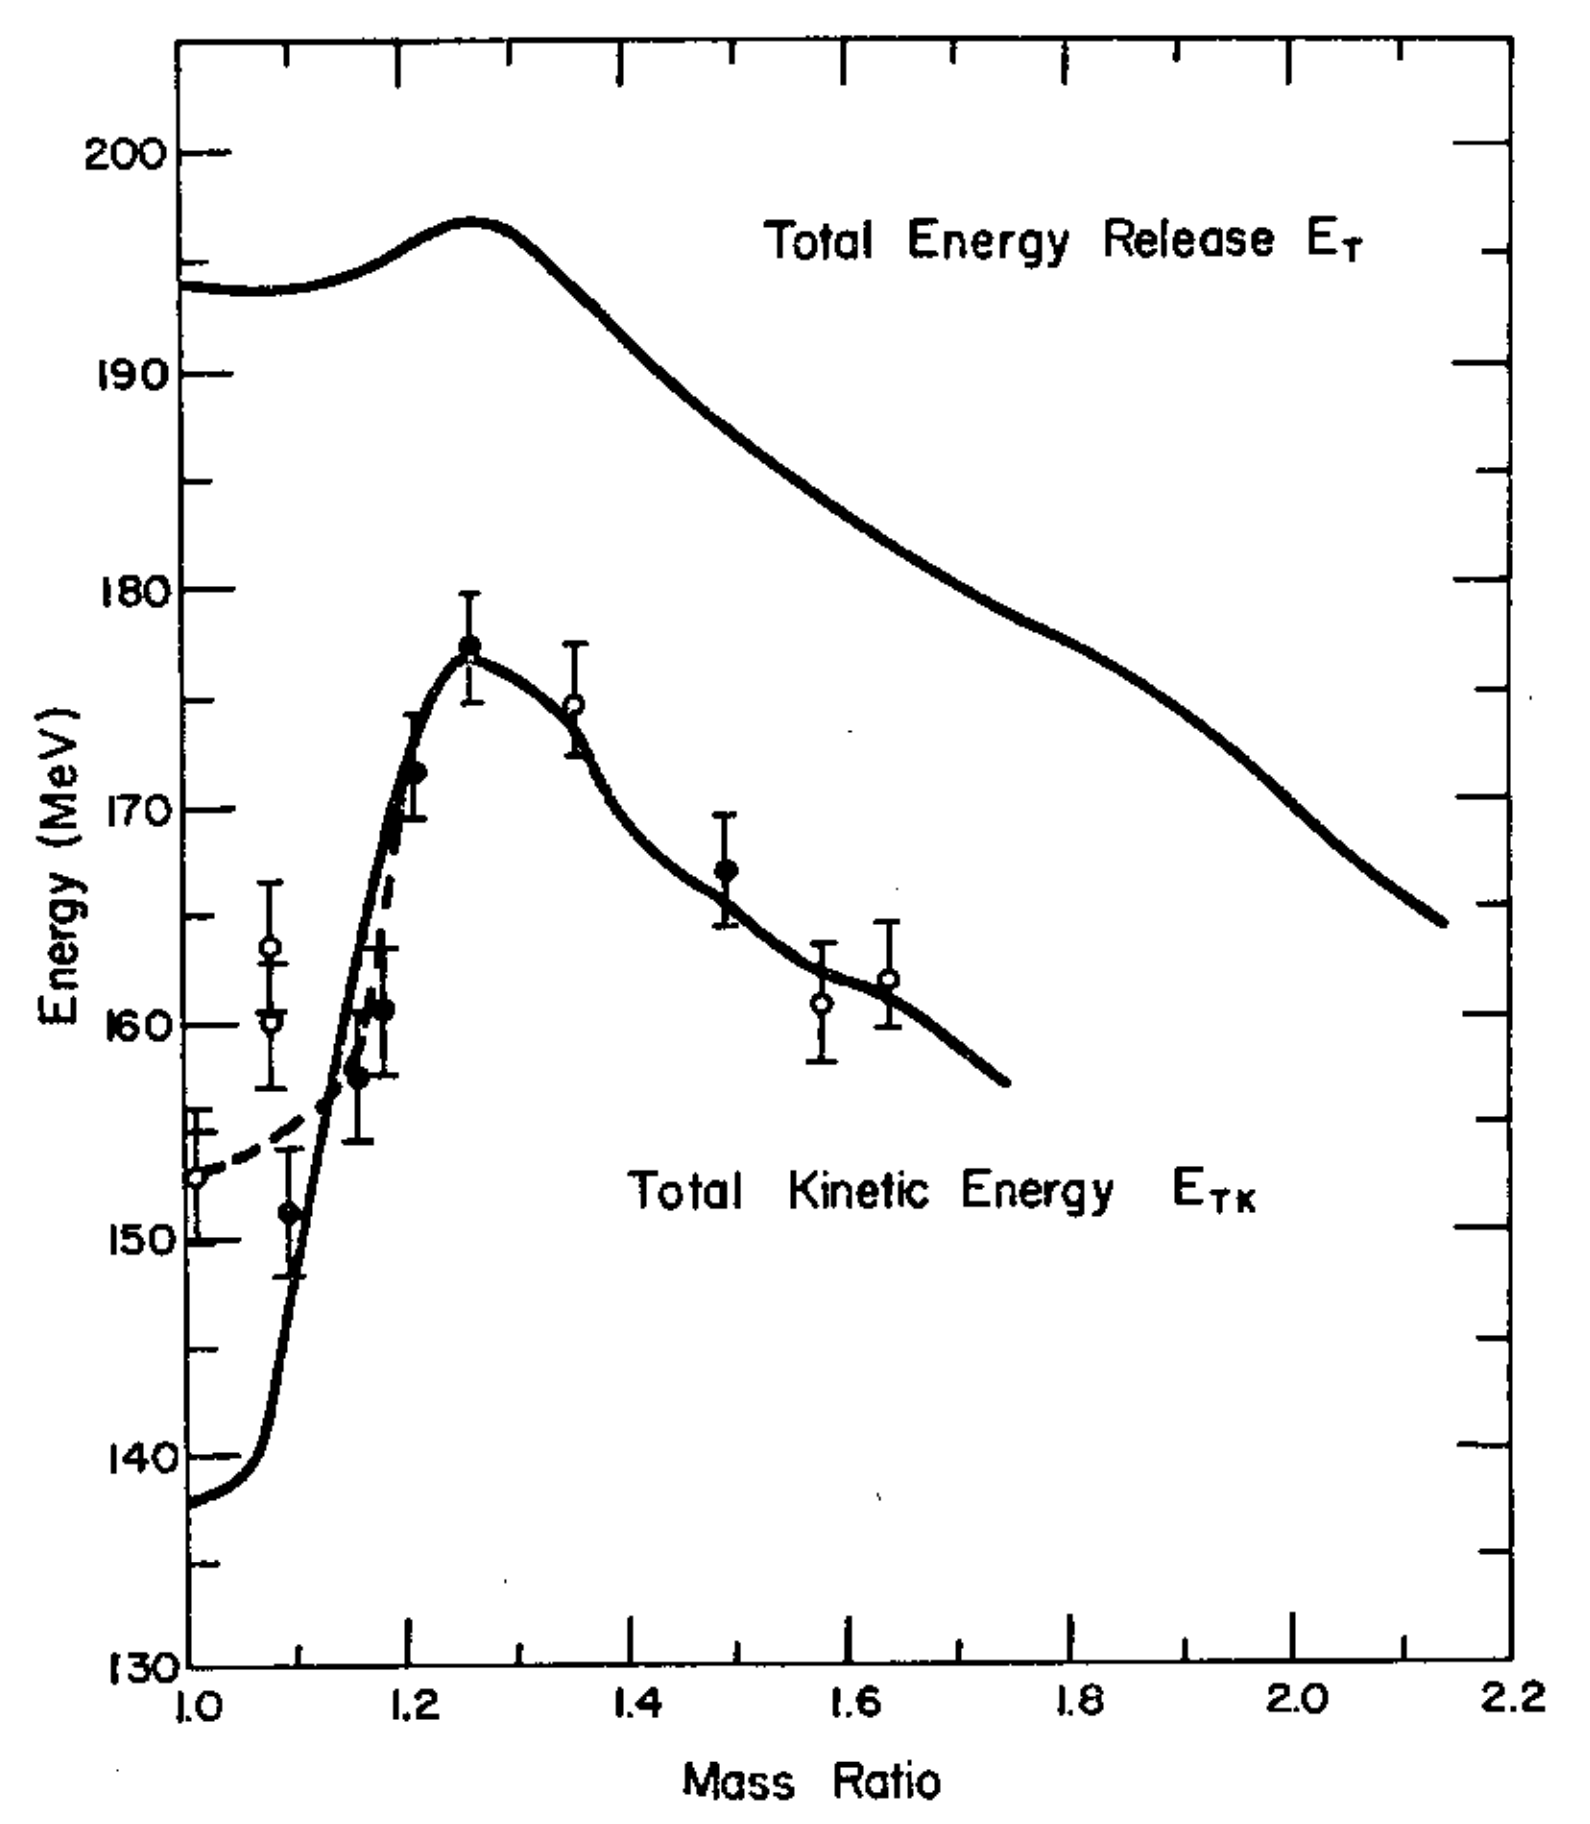
\includegraphics[height=11cm]{images/fission_energy_total.png}
\caption{Energy from thermal fission of U-235 as a function of mass ratios of child nuclei. Total energy release includes contributions from gamma rays and subsequent radioactive decays. Taken from \cite{aras1965ranges}.}
\label{figure:fissionenergy}
\end{figure}

Combustion-based power as a technology has matured over hundreds of years, with modern optimisations only looking to offer fractional percent gains in efficiency. By comparison, nuclear power technology is far from mature, with large improvements yet to be realised. One such feature is load-following, an enormously useful feature for a power plant which is currently unavailable in nuclear reactors. The biggest hurdle to achieving load-following in nuclear reactors is the issue of pellet-cladding interaction (PCI), which is the basis of the work in this thesis.

\subsection{Fission}

Commercial nuclear power plants extract energy through the process of fission, where a large nucleus is split into smaller nuclei. While it is also possible to extract energy from certain nuclei by the process of fusing them into larger ones, no fusion reactor currently exists which achieves a net positive energy output. At a fundamental level, both of these processes rely upon mass-energy equivalence. The relationship between mass and energy is shown using Einstein's famous equation:

\begin{equation}
\label{emc2}
    E = mc^{2}
\end{equation}

where $E$ is the energy of the system, $m$ is the mass and $c$ is the speed of light. Using this equation we can analyse a typical fission reaction:

\begin{equation}
\label{fission}
    U^{235}_{92} + n^{1}_{0} \longrightarrow I^{132}_{53} + Y^{101}_{39} + 3n^{1}_{0} 
\end{equation}

While the number of protons and neutrons are conserved throughout the reaction, a quick calculation will show that there is actually less mass in the products than the reactants by approximately 0.188 amu (3.127$\times 10^{-28}$ kg). This missing mass, known as the \emph{mass defect}, is converted to energy ($\sim$175 MeV). In this way, the total mass-energy of the system is conserved. 

This change in mass arises due to the phenomenon of \emph{binding energy}. In order for two or more nucleons to be thermodynamically stable when bound together, the total free energy of the bound configuration must be less than the sum of constituent nucleon free energies. Much like with energy stored in a chemical bond, the binding energy represents the energy required to separate the nucleus into individual protons and neutrons. 

Larger nuclei will generally have a greater total binding energy value compared to smaller nuclei, but the mass defect per nucleon will not necessarily be greater in a larger nucleus. It is therefore useful to normalise the binding energy by the mass number. Different isotopes have different binding energies, and any nuclear reaction which increases the binding energy per nucleon will be exothermic, whether by fission or fusion. Figure \ref{figure:bindingenergy} shows a plot of binding energy per nucleon against mass number with the relevant isotopes from Equation \ref{fission}. 

%235.0439299 + 1.008664 (236.0525939) -> 131.907997 + 100.93031 + 3.025992 (235.864299)



\begin{figure}[htp]
\centering
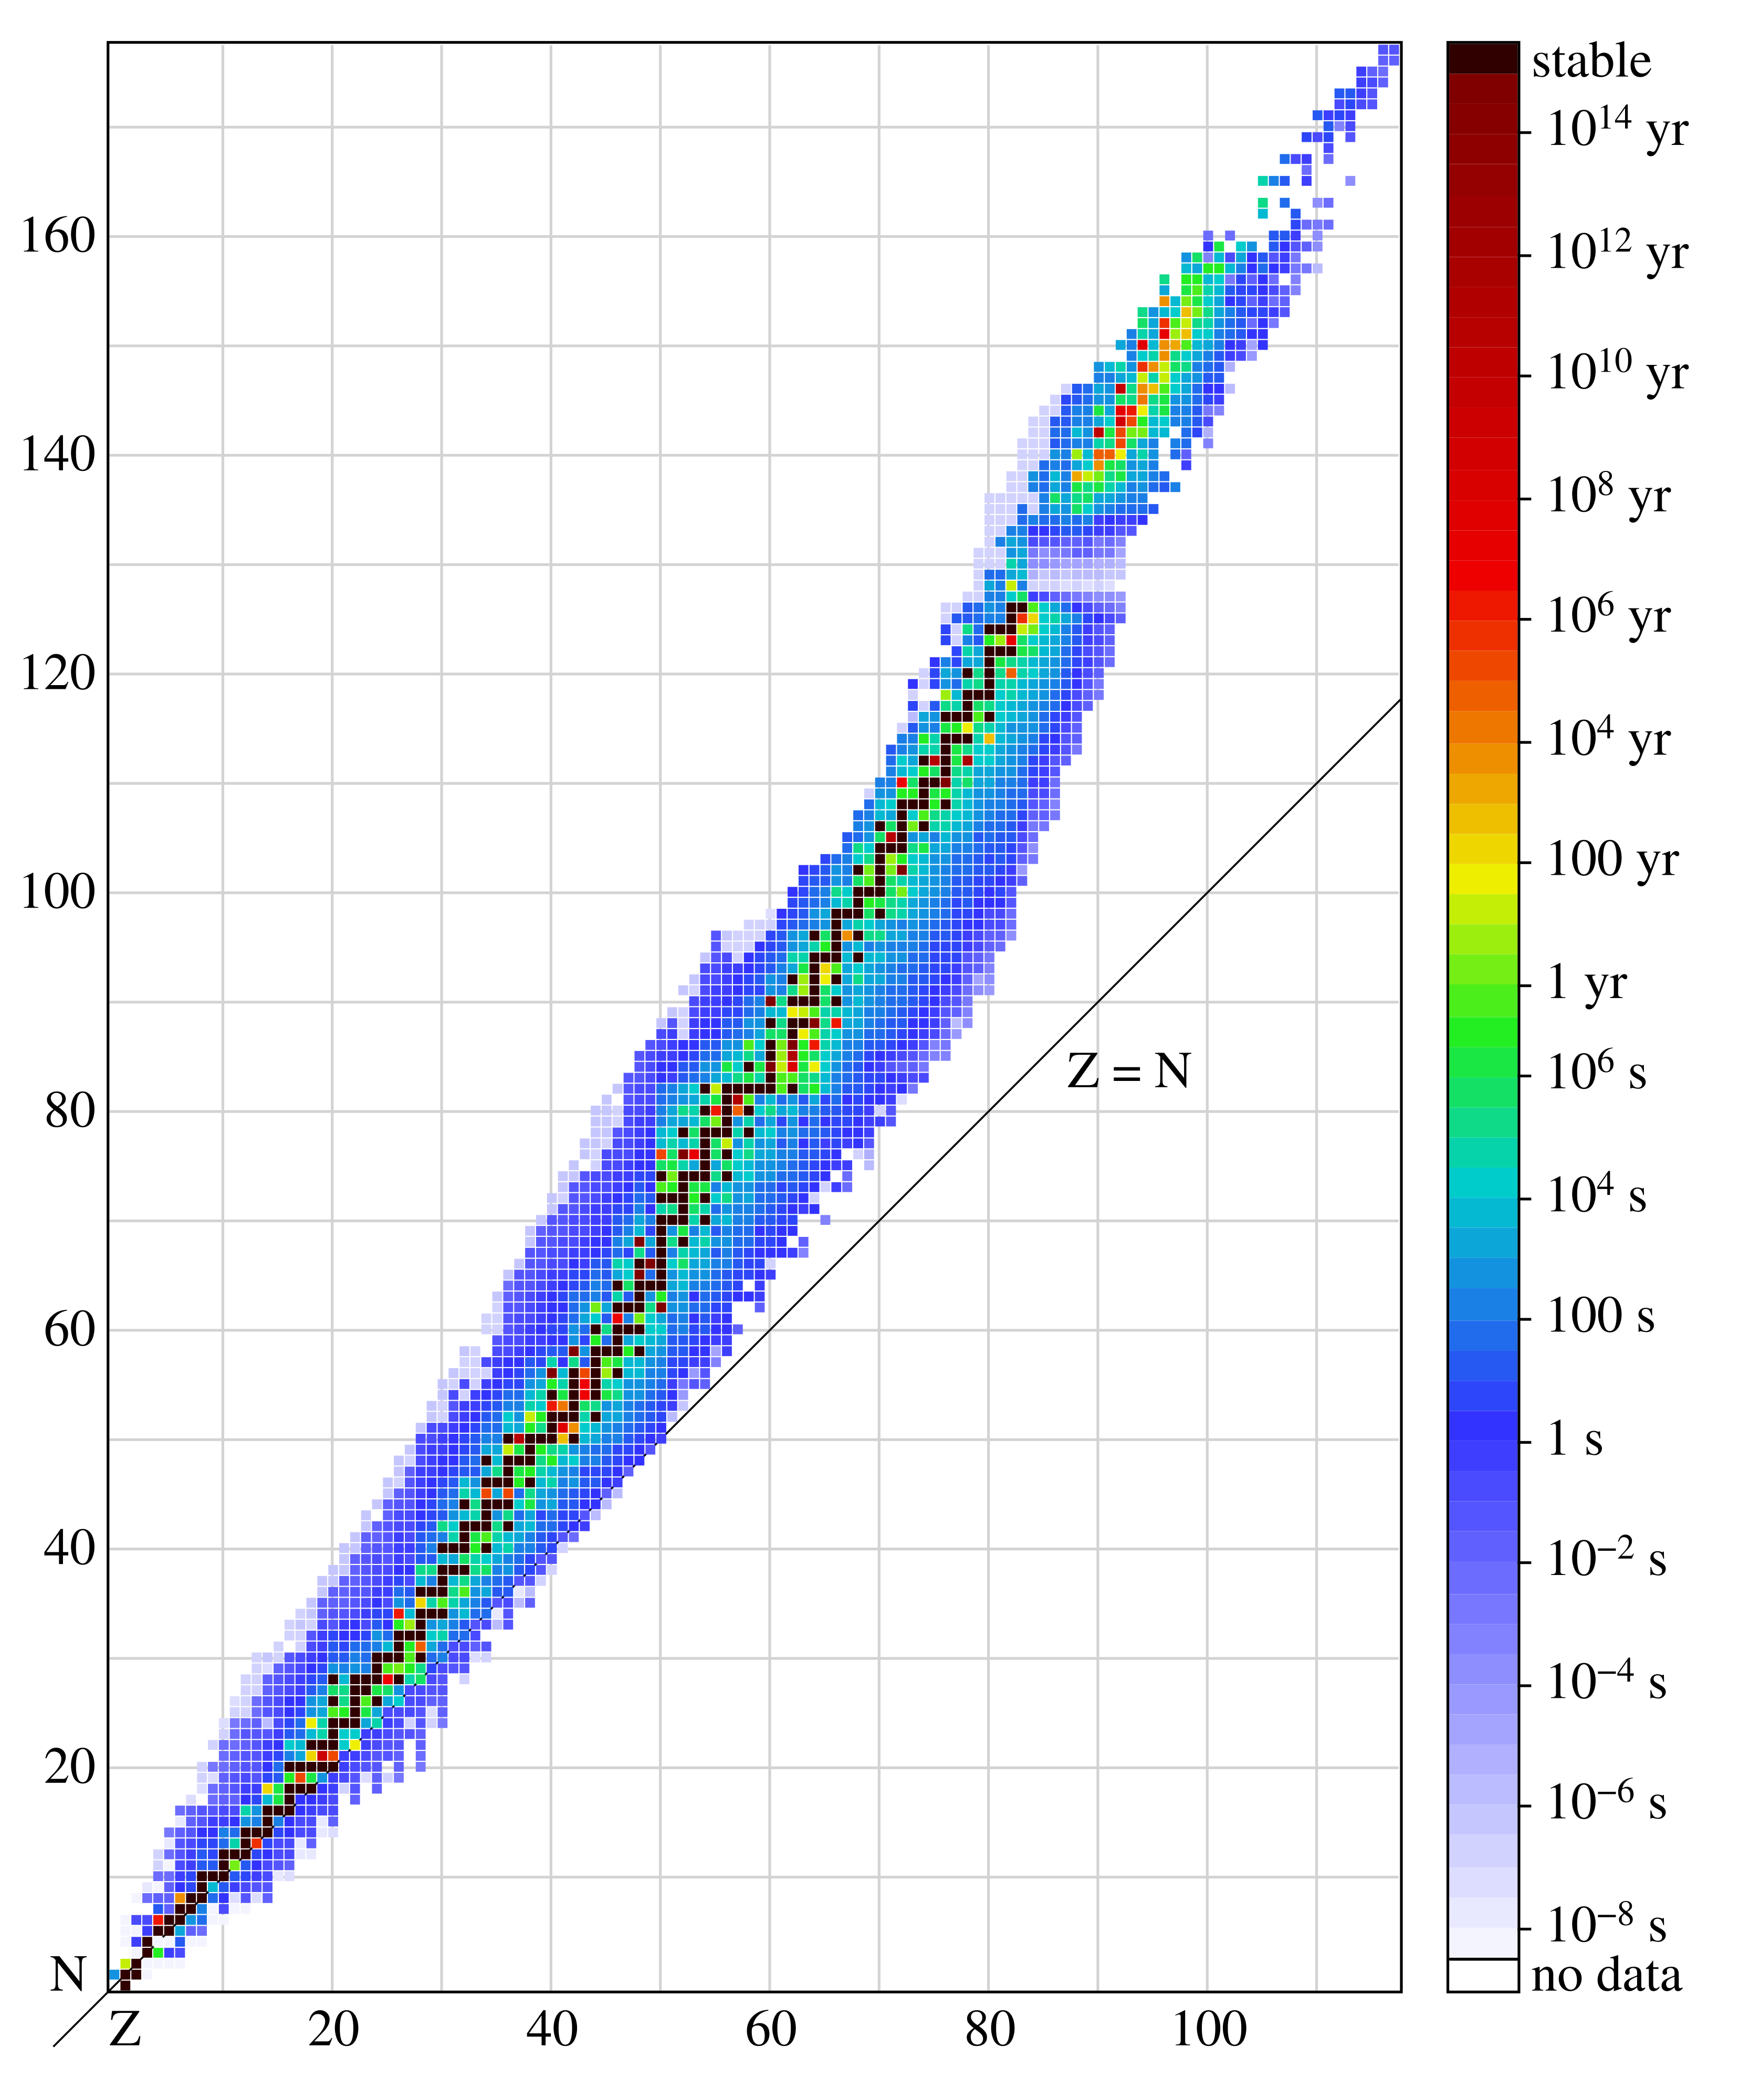
\includegraphics[height=11cm]{images/Isotopes_and_half-life.png}
\caption{Plot of neutron number against proton number for nuclei with half-lives greater than 10${^{-4}}$s. Half-life of the dominant decay mode is shown. Taken from \cite{BenRGPlotIsotopes}.}
\label{figure:NZcurve}
\end{figure}

\begin{figure}[htp]
\centering
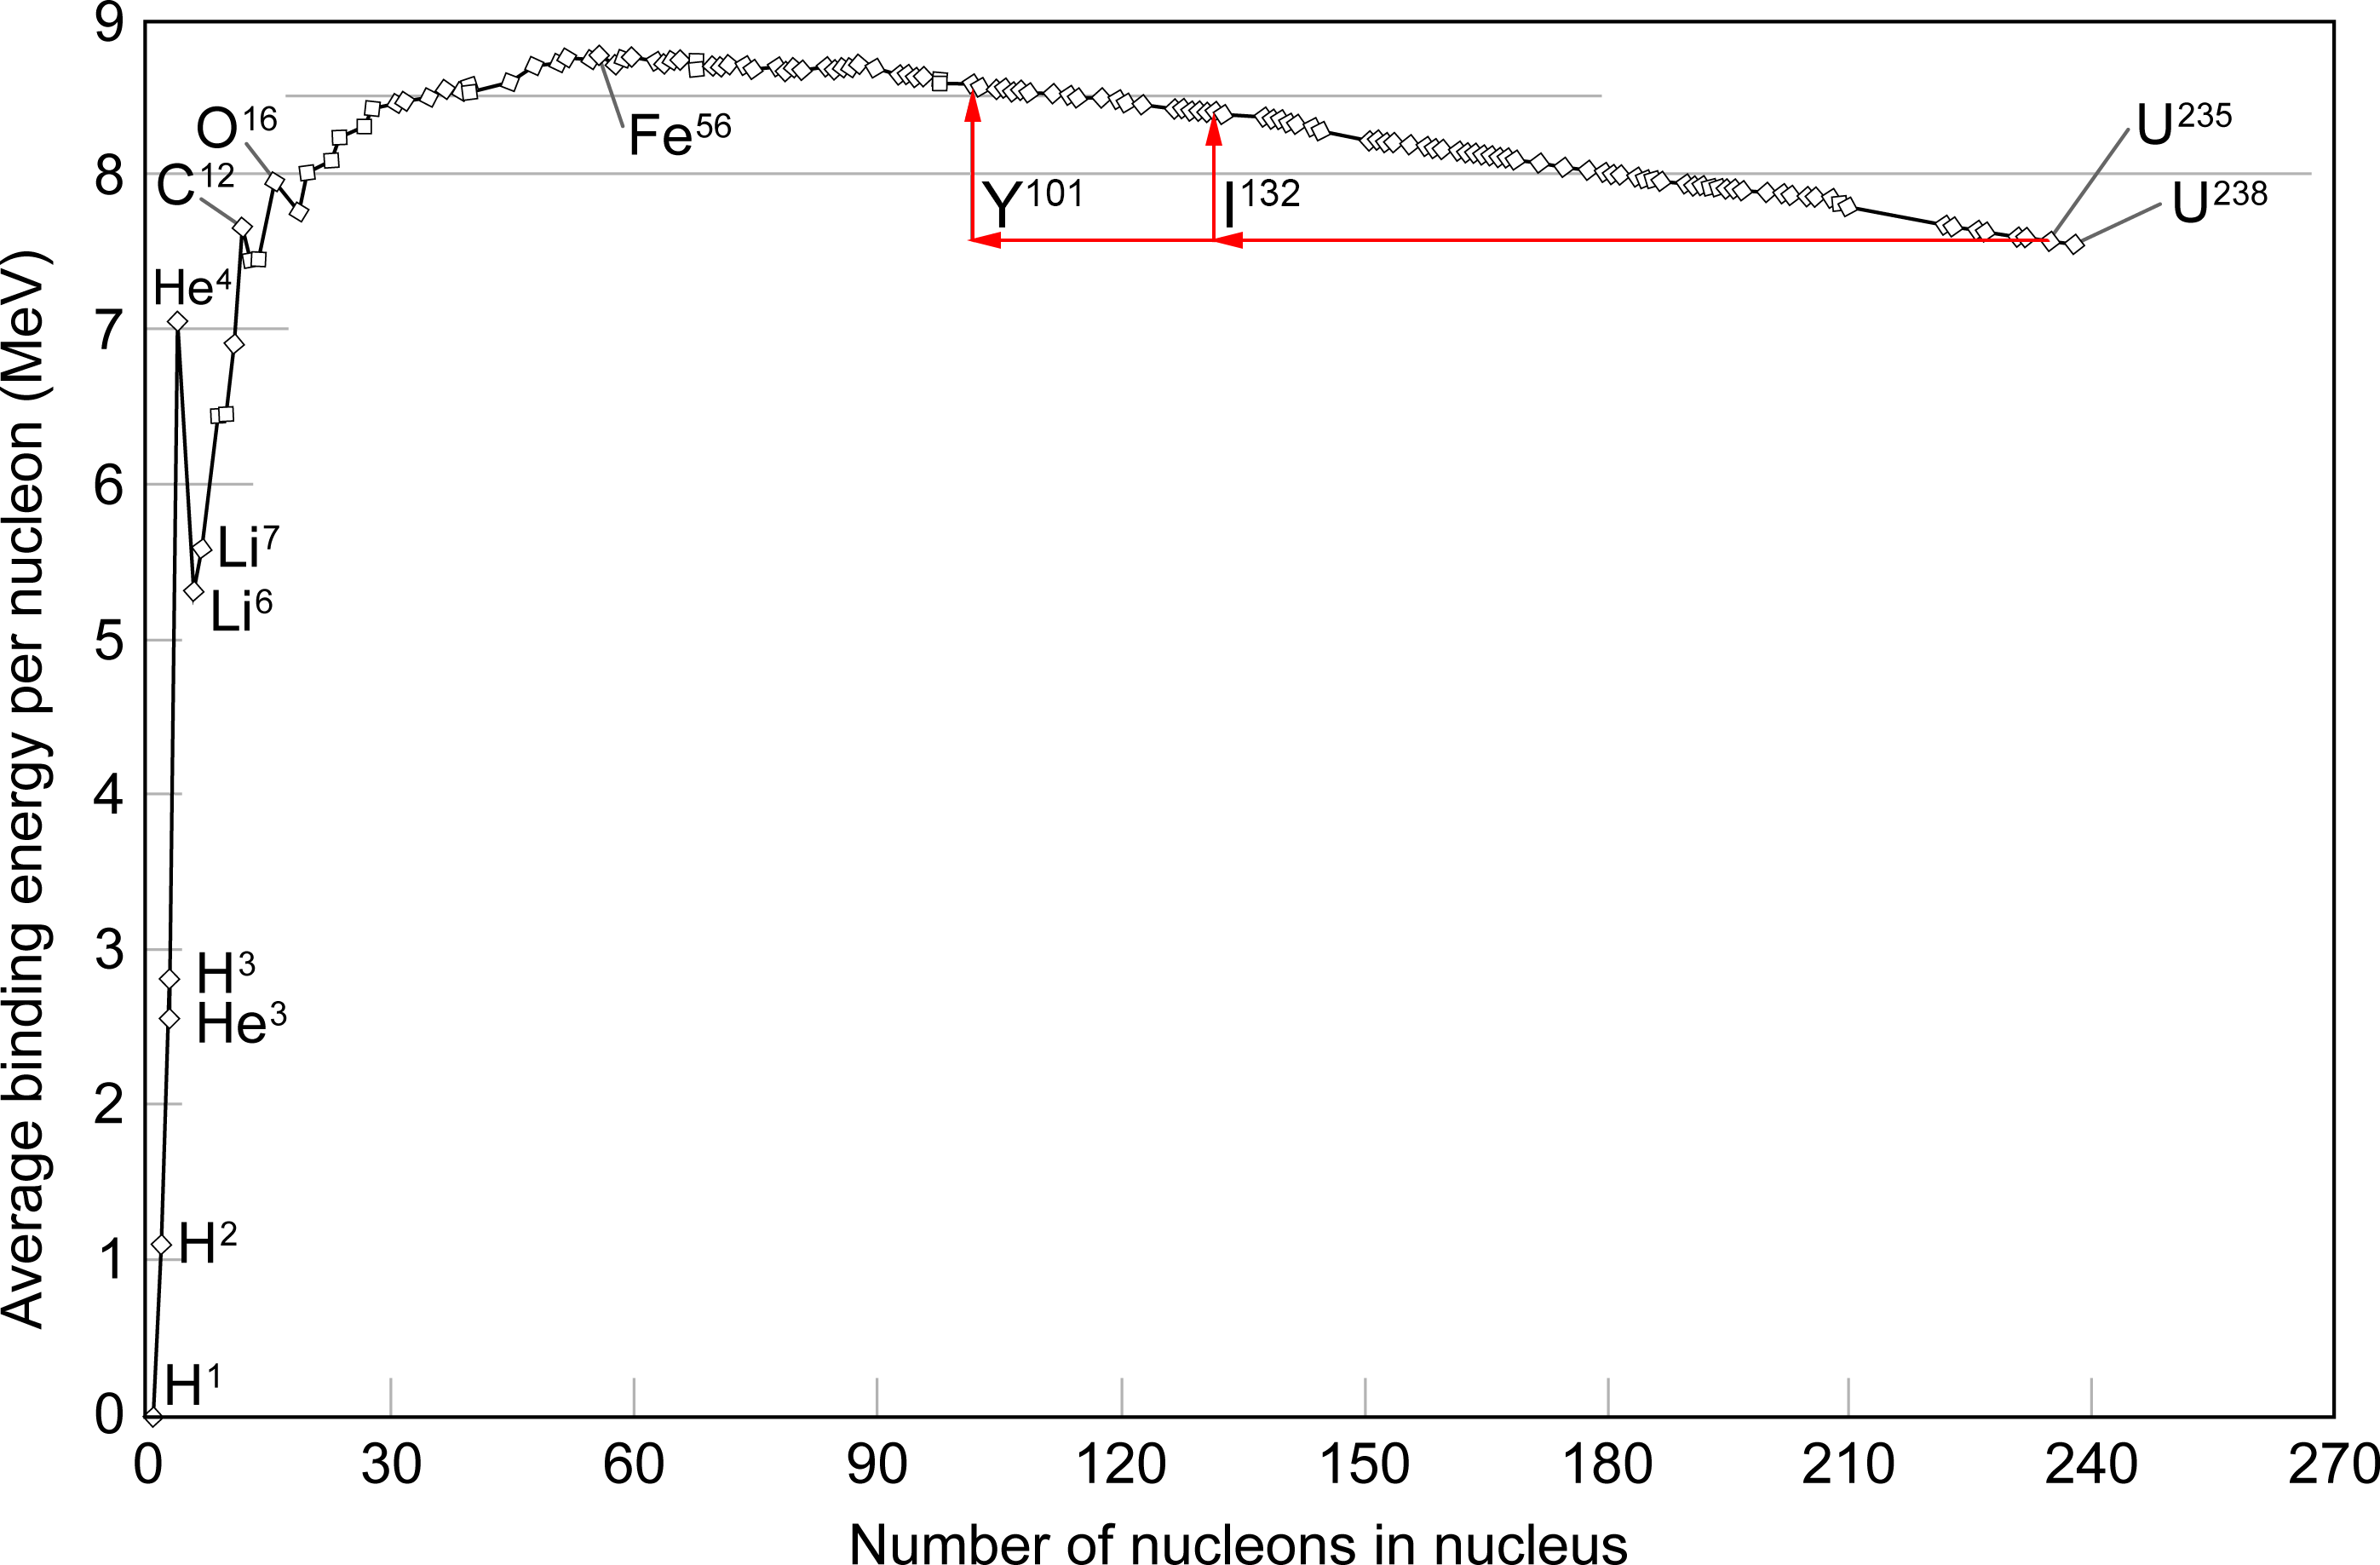
\includegraphics[height=11cm]{images/Binding_energy_curve.png}
\caption{Plot binding energy per nucleon against mass number. Arrows indicate the reaction shown in equation \ref{fission}. Adapted from \cite{FastfissionBindingCurve}.}
\label{figure:bindingenergy}
\end{figure}


\subsection{Reactor design}

Commercial nuclear reactors are large boilers in a Rankine cycle, designed to maximise heat transfer to a working fluid. All nuclear plants use steam turbines on the generation side, though the reactor coolant may be another fluid in a separate loop, such as carbon dioxide in gas-cooled reactors (GCRs), or even in a separate water loop such as in pressurised water reactors (PWRs) and CANDU. The work in this thesis is focused on zirconium-based claddings which are used worldwide in all commercial reactors except GCRs and sodium-cooled fast reactors. The most prevalent reactor type is the PWR, followed by the boiling water reactor (BWR) {REFER TO TABLE}. 


%Depending on the type of reactor, one or two coolant loops may be utilised. The generation side always involves 

\begin{itemize}
\item LWRs vs other kinds of reactors
\item Zirconium cladding used because of strength + low thermal neutron abs cross section
\item Thermal energy transferred from fuel to coolant
\item RPV is pressurised to 150 bar in PWRs, less in BWRs and even less in CANDU
\end{itemize}

\subsection{Nuclear reactor fuel pins}

Fuel assemblies in nuclear reactors are bundles of fuel pins. In most commercial reactors, these fuel pins are comprised of a zirconium-based cladding which is filled with UO$_{2}$ fuel pellets, each of which are approximately 1 cm$^{3}$ in volume. Once loaded with fuel pellets, the fuel pins are capped and filled with inert helium gas, pressurised to between 2 and 25 atm to improve heat transfer from the fuel pellets to the coolant as well as delaying inward creep deformation of the cladding due to the high coolant pressure \cite{King1980}. In the early stages of a fuel pin's life, there is a small gap between the fuel pellet and the cladding, known as the pellet-cladding gas gap. This gas gap slowly closes with increasing burn-up mostly due to swelling of the fuel pellets.

\subsubsection{Zirconium cladding}



\begin{itemize}
\item Zirconium cladding
\item Ceramic fuel pellets
\item Pellet-cladding gas gap
\item Cladding failure (great review here \cite{alam2011review})
\end{itemize}

\subsection{Effects of radiation on materials}

While ionising radiation is always present in the environment as background radiation, the intensity of radiation in a nuclear reactor is so great that it presents significant engineering challenges because of how it affects different materials.

Radiation hardening (also known as radiation embrittlement) is a phenomenon which affects most materials subjected to ionising radiation. It is characterised by a loss of plasticity caused by radiation damage over time, leading to an increased risk of cracks and failure of components. While zirconium is a very useful nuclear material due to it's neutron transparency, it is still susceptible to this type of damage \cite{Wisner1998CombinedZircaloy-2}. Beyond certain levels of radiation damage, phase changes may also occur. In \zirconia\ however,  

Amorphisation is another effect of radiation damage. This is characterised by a loss of long-range order of atoms in a crystal. This typically occurs beyond a certain threshold of radiation damage depending on the material, called the critical amorphisation dose. Amorphisation is problematic because the loss of a defined crystal structure results in both a reduction in structural stability (amorphous materials have a higher Gibbs free energy than their crystalline counterparts) and causes swelling of the material. In the literature, there is evidence of amorphisation in cubic stabilised \zirconia\ when bombarded with Cs$^{+}$ ions up to a fluence of $1 \times 10^{21}$ ions m$^{-2}$ \cite{amorphization2000wang}. However, no amorphisation is seen at an Xe$^{2+}$ fluence of $2 \times 10^{21}$ ions m$^{-2}$, or an I$^{+}$ fluence of $5 \times 10^{19}$ ions m$^{-2}$ \cite{sickafus1999radiation}.

One material phenomenon exclusive to nuclear reactor environments is neutron activation. The high free neutron environment leads to neutron capture in various nuclei within the reactor, including those of the fuel assemblies, coolant and RPV. There are many possible (n,x) reactions that may occur in materials experiencing a neutron flux, but of particular concern is transmutation of nuclei following a nuclear capture event. When a stable nucleus captures a neutron and becomes unstable, the nucleus may then emit particles to reduce it's free energy, altering it's atomic number in the process. This new element will have different chemical properties compared to the parent nucleus by virtue of a different electronic structure. This will change the elemental composition of a material, typically in an unfavourable way with dopants that negatively affect some desired material property. The extremely large number of nuclei relative to neutron flux means that this effect is small, though over time this becomes more significant due to accumulation of these dopant elements.

\begin{itemize}
\item Radiolysis
\end{itemize}

\subsection{Fission products, their distribution and decay chains}

\begin{itemize}
\item Bi-modal distribution of fission products due to binding energy gains (get a good binding energy per nucleon plot)
\item Fission products are almost always neutron-rich and will decay by beta-
\item Iodine is always paired with yttrium (53+39 protons). Yttrium happens to be a very good cubic phase stabiliser in \zirconia\ and decays into Zr.
\item Iodine appears both from direct fission, and from decay of tellurium which is also a common fission product.
\item The decay chain we are interested in is Te -> I -> Xe -> Cs
\end{itemize}

\section{Pellet-cladding interaction (PCI)}

PCI has been known about since 1974. Many studies and reviews have been made \cite{alam2011review}

\subsection{Effect of power ramps}
B.Cox PCI failures of Zr alloy fuel cladding \cite{bcoxpelletclad1990} talks about how they found out that fission products were necessary for PCI failures on page 260 (citation 54)

\subsection{Pellet-clad gap and bonding}

\begin{itemize}
\item At the beginning of life, there is a gas gap between the fuel pellet and the cladding, typically filled with an inert gas like helium during the manufacturing process.
\item With increasing burnup, radiation damage in the fuel pellet causes it to swell and therefore reduce the pellet-cladding gap, eventually making contact (and exerting a force) with the cladding.
\end{itemize}

\subsection{Iodine corrosion of zirconium}

\section{Oxidation of zirconium}

The oxidation of zirconium to produce \zirconia\ occurs during manufacture of the fuel clad when the metal is exposed to oxygen in air. \zirconia\ is a ceramic with material properties that make it desirable in many industrial applications, including solid-oxide fuel cells \cite{radford1979zirconia}, refractory linings \cite{whittemore1952fused}, and nuclear waste storage \cite{wang2012ceramics}.

\subsection{Oxygen solubility of zirconium}

\begin{itemize}
\item Oxygen is soluble in zirconium up to 29\% molar mass at "insert temperature".
\item Several PCI studies have assumed a mechanism whereby the \zirconia\ layer is fractured, allowing iodine to attack fresh metal surface, but these studies always assume that the exposed metal is oxygen-depleted.
\item It is not oxygen depleted, therefore they will always overestimate the amount of oxygen necessary to form a new passive oxide layer.
\end{itemize}

\subsection{Oxide growth mechanism}

An oxide layer will typically form on the surface of zirconium metal even at very low oxygen partial pressures \cite{causey2005review}. The oxidation process is mainly driven by the ingress of oxygen ions. Initially, the oxide is highly protective, growing slowly into the metal until it reaches a thickness of approximately 2-3 $\mu$m \cite{garzarolli1991oxide,dawson1968kinetics}, after which the oxide growth mechanism enters a `post-transition' stage where the oxidation kinetics follow a cubic-rate law  \cite{porte1960oxidation}.

\subsection{Outer oxide vs inner oxide}
The fuel cladding of an LWR develops an oxide on both the inner and outer surfaces due to exposure to oxygen in air during manufacture. 
\subsection{Sources of oxygen}

\begin{itemize}
\item Initial oxidation occurs due to exposure to oxygen in air during manufacturing
\item Evolution of oxygen from UO2 fuel pellet
\end{itemize}


While \zirconia\ would ideally adopt the regular cubic fluorite structure, we only observe cubic stabilisation at elevated temperatures where the ionic radii of the zirconium ion increases (and possibly a stabilising phonon mode contribution). Yttrium is known to stabilise the cubic phase in \zirconia\ at standard conditions. This is accomplished by substituting a Zr\textsuperscript{4+} ion with Y\textsuperscript{3+} and the binding of two neighbouring oxygen vacancies, effectively producing a sub-unit of yttria (Y\textsubscript{2}O\textsubscript{3}) in the \zirconia\ lattice. This stabilising effect is observed because the yttrium ion is of the appropriate size to maintain the oxygen ions and vacancies in the VIII coordination at low temperatures, as can be seen from ionic radii values in Table \ref{figure:ionicradii}. 

\begin{table}[htp]
\onehalfspacing
\centering
\caption{Ionic radii of Zr\textsuperscript{4+} and Y\textsuperscript{3+} in various coordination environments. Values taken from \cite{Shannon1976}.}
\label{figure:ionicradii}
\begin{tabular}{ccc}
\hline
Ion & Coordination & Ionic Radius (\r{A}) \\ \hline
\multicolumn{1}{c}{\multirow{6}{*}{Zr\textsuperscript{4+}}} & \multicolumn{1}{c}{IV} & 0.59 \\
\multicolumn{1}{c}{} & \multicolumn{1}{c}{V} & 0.66 \\
\multicolumn{1}{c}{} & \multicolumn{1}{c}{VI} & 0.72 \\
\multicolumn{1}{c}{} & \multicolumn{1}{c}{VII} & 0.78 \\
\multicolumn{1}{c}{} & \multicolumn{1}{c}{VIII} & 0.84 \\
\multicolumn{1}{c}{} & \multicolumn{1}{c}{IX} & 0.89 \\ \hline
\multicolumn{1}{c}{\multirow{4}{*}{Y\textsuperscript{3+}}} & \multicolumn{1}{c}{VI} & 0.90 \\
\multicolumn{1}{c}{} & \multicolumn{1}{c}{VII} & 0.96 \\
\multicolumn{1}{c}{} & \multicolumn{1}{c}{VIII} & 1.019 \\
\multicolumn{1}{c}{} & \multicolumn{1}{c}{IX} & 1.075 \\ \hline
\end{tabular}
\end{table}

\begin{figure}[htp]
\centering
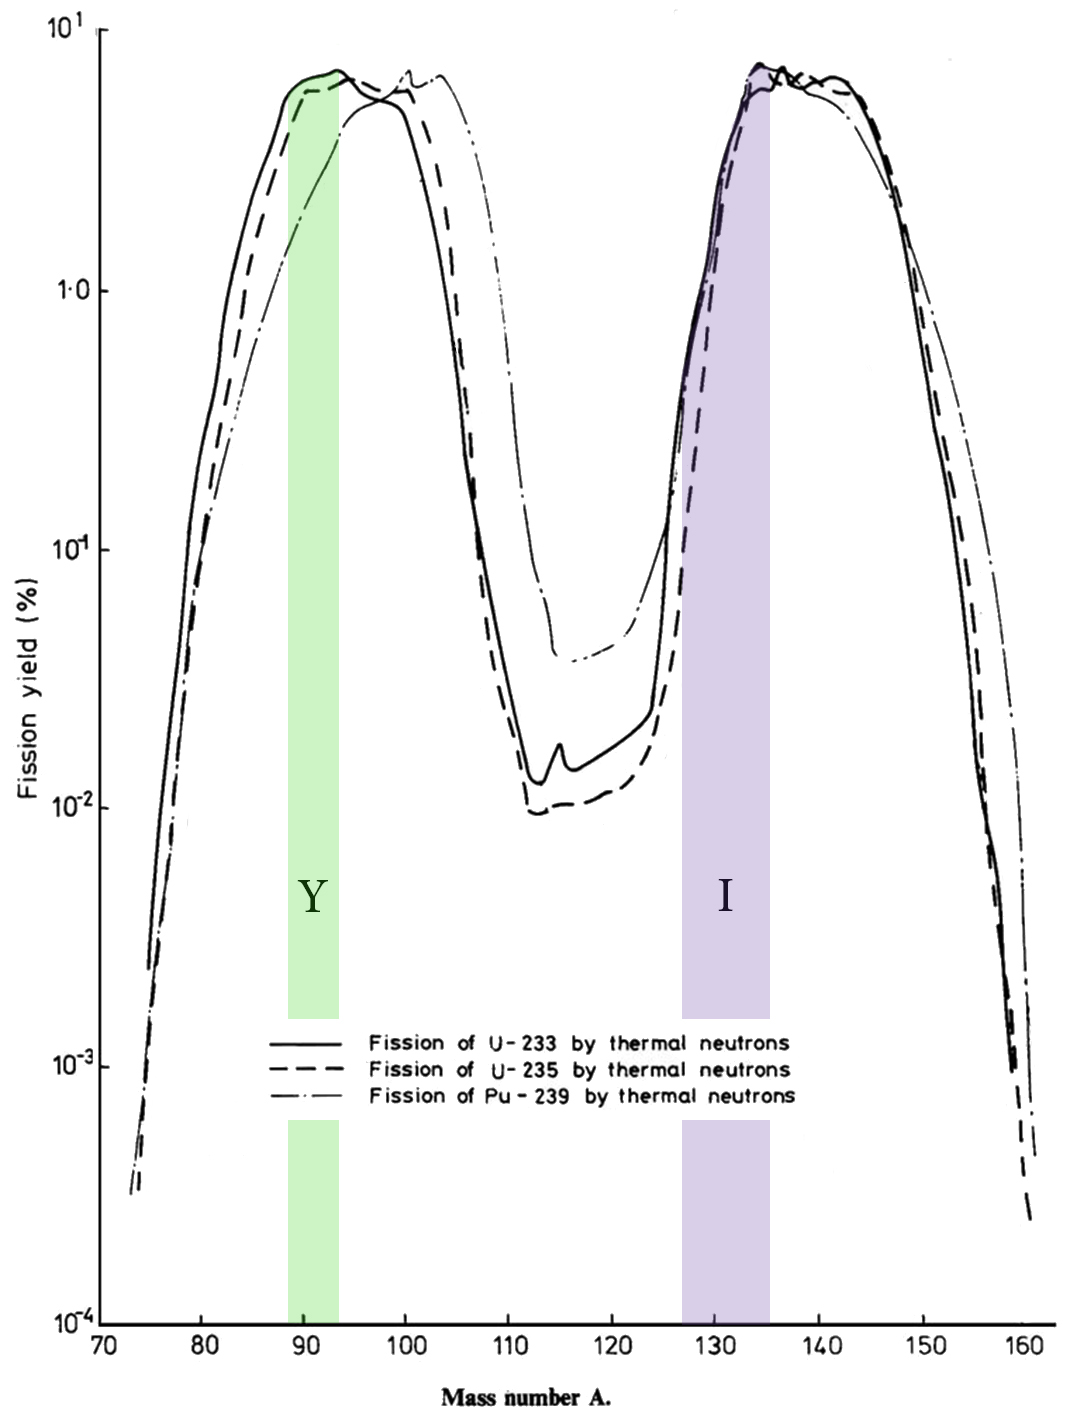
\includegraphics[height=11cm]{images/fissionyield.jpg}
\caption{Plot of the percentage yield of nuclei with a given mass following a fission event. Range of masses corresponding to isotopes of iodine shown in purple and isotopes of yttrium shown in green.}
% M. F. James, R. W. Mills and D. R. Weaver (1991) UKAEA Reports, AEA-TRS-1015, AEA-TRS-1018 
         %  and AEA-TRS-1019.
\label{figure:fissionyield}
\end{figure}

\subsection{Cubic phase stability}

\begin{itemize}
\item The existence of a cubic phase in undoped \zirconia\ is debated. The high temperatures required for stabilisation of the cubic phase and the similarity to the tetragonal phase make it difficult to discern as a third phase.
\item Also due to the high temperature, the stability of the cubic phase in DFT calculations may be inaccurate. This is discussed further in Chapter 3.
\end{itemize}

\begin{figure}[htp]
\centering
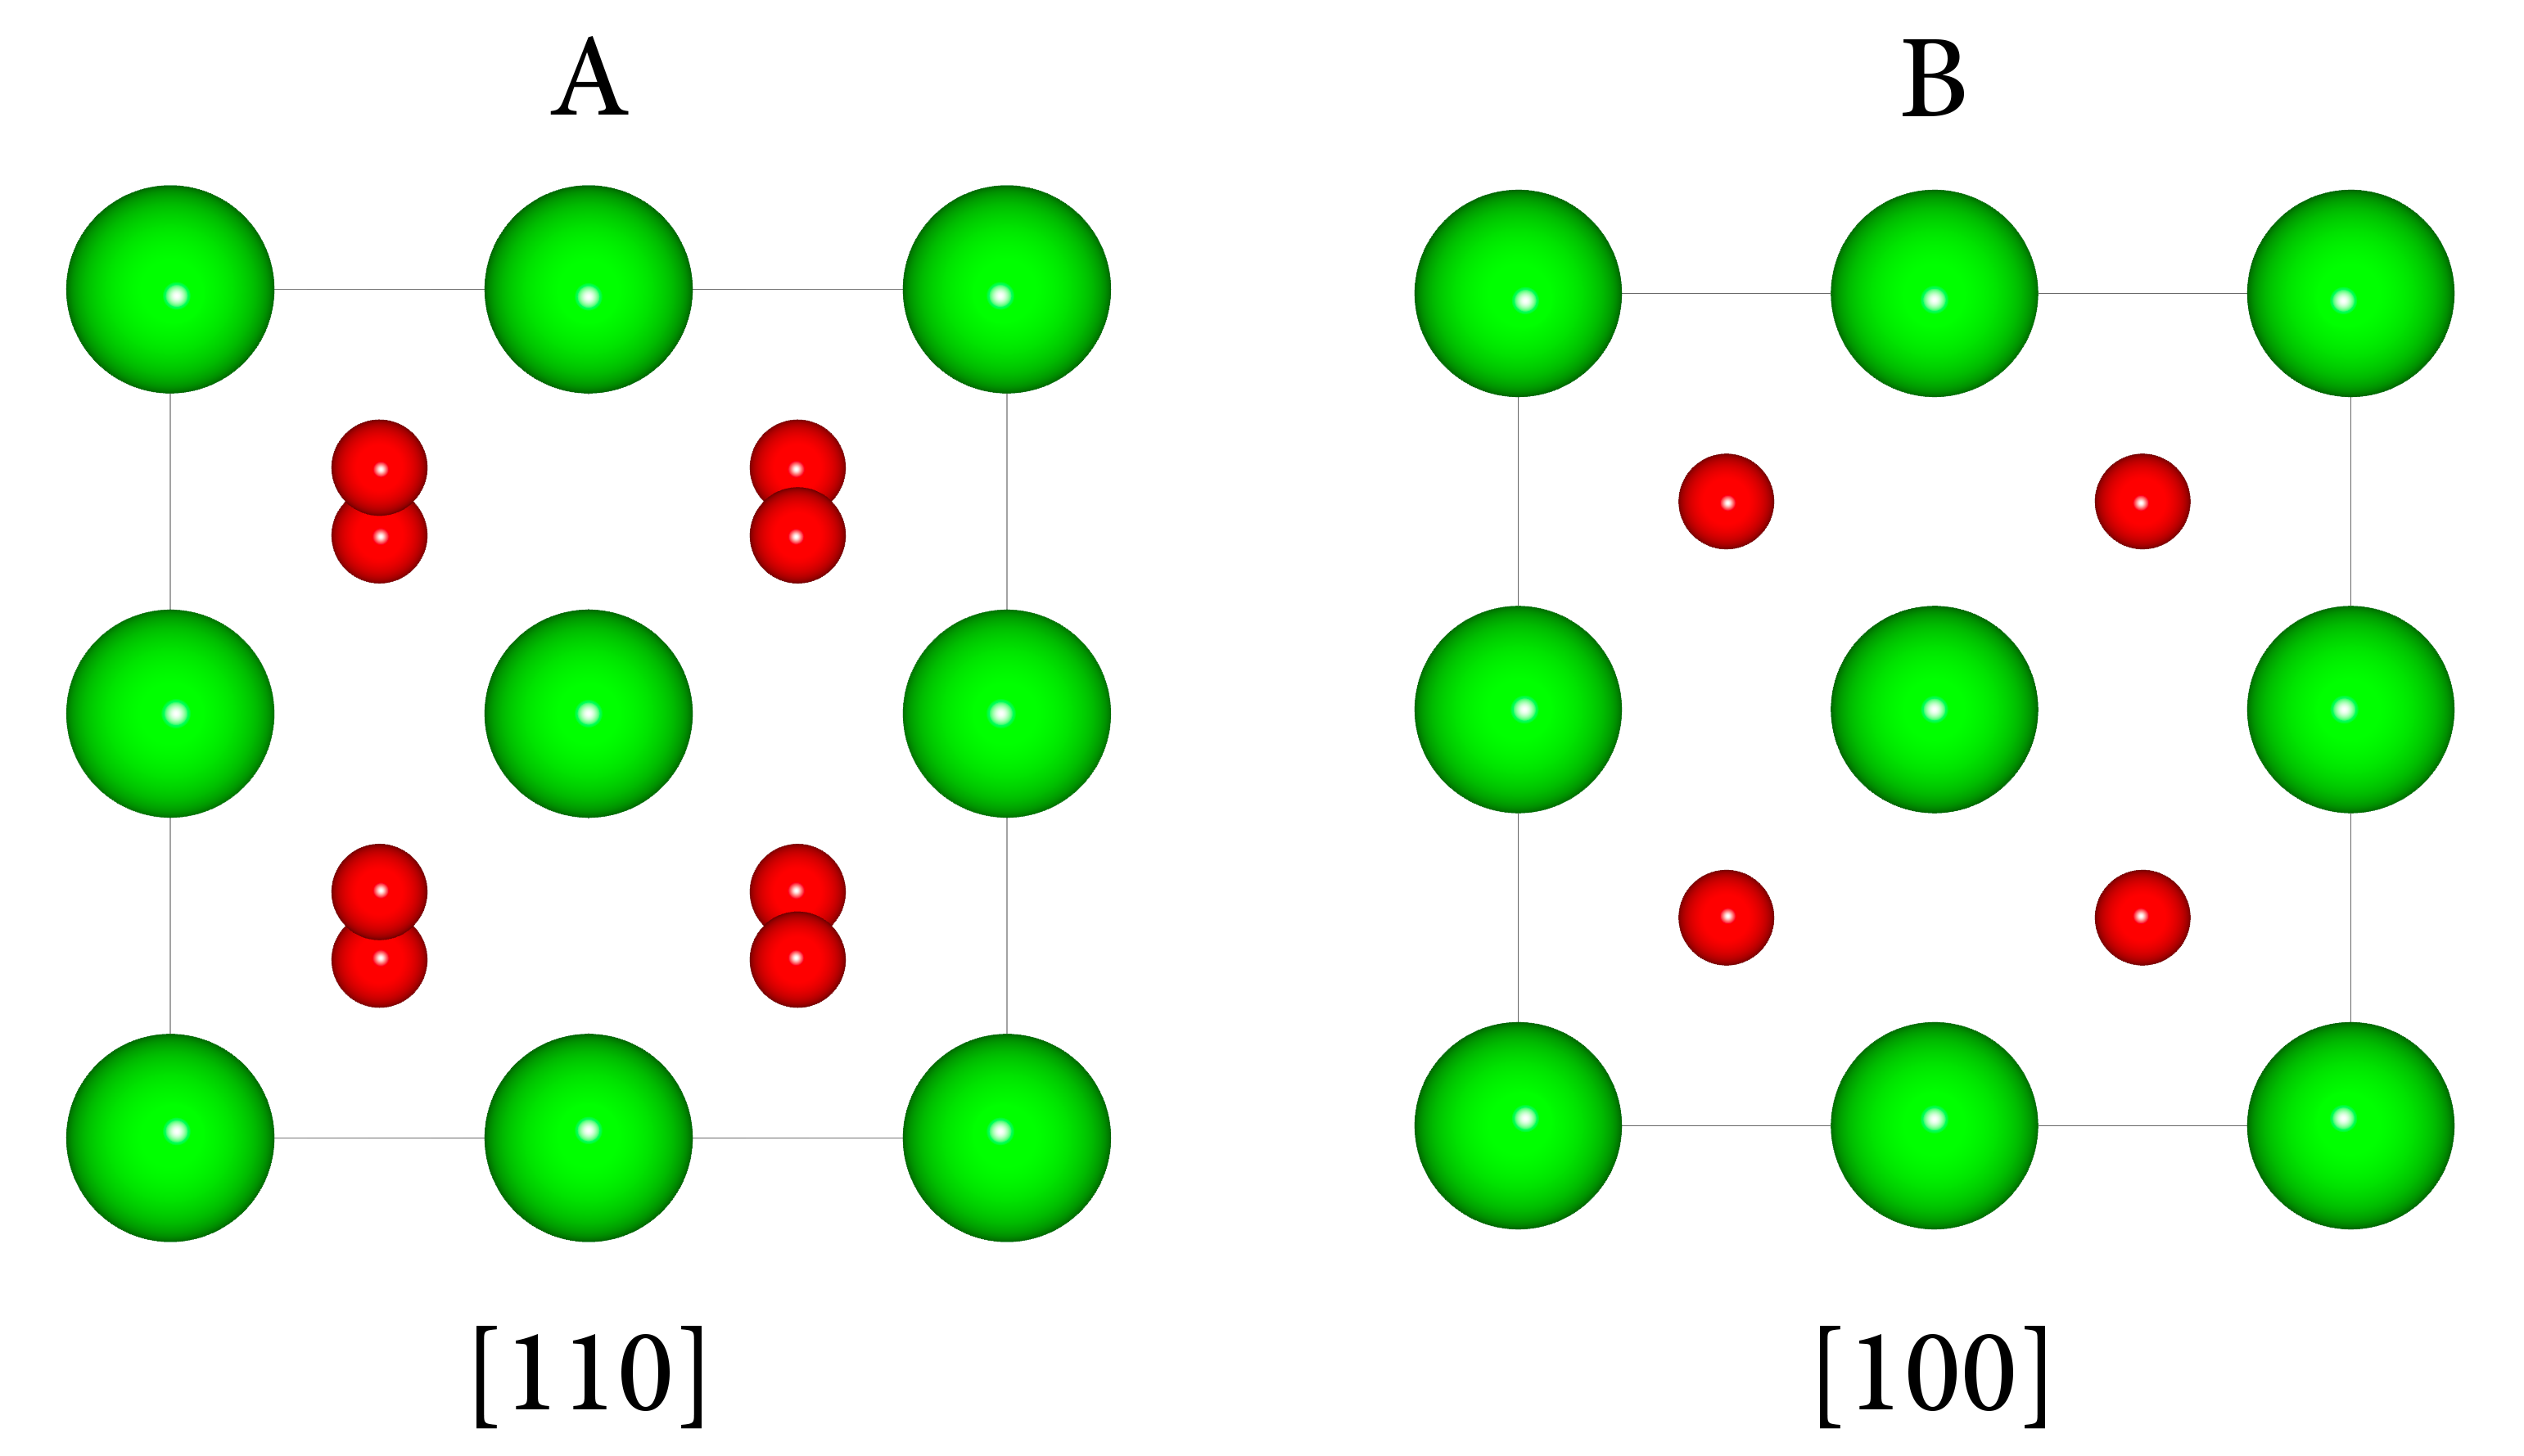
\includegraphics[height=7cm]{images/tet_vs_cubic.png}
\caption{\textbf{A}) Tetragonal \zirconia\ viewed along the [110] direction. \textbf{B}) Cubic \zirconia\ viewed along the [100] direction. Zirconium atoms are shown in green and oxygen atoms in red.}
\label{figure:tetvscubic}
\end{figure}

\section{Atomistic Simulation}

\subsection{Classical approach - molecular dynamics}

\begin{itemize}
\item Molecular dynamics allows for large system sizes (millions of atoms) compared to DFT because of the low computational cost of classical potentials. 
\item These are mainly pair potentials (although many-bodied potentials are also used) which are some combination of a short-range repulsion term (Pauli exclusion, nuclear repulsion if van der waals is taken into account) and a long range Coulombic attraction term
\end{itemize}

\subsection{Quantum mechanical approach - DFT}

\begin{itemize}
\item Up to hundreds of atoms, but far more fundamental data such as electron density.
\item Very computationally expensive, but with clever workarounds for bulk crystallographic systems.
\end{itemize}

\subsection{Band gap}

\begin{itemize}
\item Electron energy levels are quantised.
\item In a crystal, large numbers of electrons and many possible configurations lead to electron energy 'bands' made up of many quantised energies (electron band theory). See http://hyperphysics.phy-astr.gsu.edu/hbase/Solids/band.html
\item Non-metals exhibit an energy gap between valence and conduction electron bands, demarcating insulators and conductors.
\end{itemize}

\begin{figure}
\begin{center}
\begin{tikzpicture}
	\begin{axis}
		[width=11cm, xlabel={Energy (eV)}, ylabel={Electronic density of states}, ymin=0, ymax=12, xmin=0, xmax=16, legend style={{draw=}, at={(0.05,0.95)}, anchor=north west, legend columns=1}]
% 		\addplot[no marks] table [x=log(pO2)/atm, y=Electrons,]{tetintrinsic.dat}; \addlegendentry{e\SPSB{$\prime$}{}};
%         \addplot[no marks, dashed] table [x=log(pO2)/atm, y=Holes, ]{tetintrinsic.dat}; \addlegendentry{h\SPSB{\textbf{\textperiodcentered}}{}};
%         \addplot[no marks, densely dotted, red] table [x=log(pO2)/atm, y=VO+2,]{tetintrinsic.dat}; \addlegendentry{V\SPSB{\textbf{\textperiodcentered\textperiodcentered}}{O}};
%         \addplot[no marks, dashed, red] table [x=log(pO2)/atm, y=VO+1,]{tetintrinsic.dat}; \addlegendentry{V\SPSB{\textbf{\textperiodcentered}}{O}};
%         \addplot[no marks, red] table [x=log(pO2)/atm, y=VO0,]{tetintrinsic.dat}; \addlegendentry{V\SPSB{$\times$}{O}};
%         \addplot[no marks, densely dotted, blue] table [x=log(pO2)/atm, y=VM-4,]{tetintrinsic.dat}; \addlegendentry{V\SPSB{$\prime\prime\prime\prime$}{Zr}};
%         %\addplot[no marks, dashed, blue] table [x=log(pO2)/atm, y=VM-3,]{tetintrinsic.dat}; \addlegendentry{V\SPSB{$\prime\prime\prime$}{Zr}};
       \addplot[no marks] table [x=mono_x, y=mono_y,]{dat/eDOS.dat}; \addlegendentry{Monoclinic};
       \addplot[no marks, dashed] table [x=tet_x, y=tet_y,]{dat/eDOS.dat}; \addlegendentry{Tetragonal};
       \addplot[no marks, densely dotted] table [x=cubic_x, y=cubic_y,]{dat/eDOS.dat}; \addlegendentry{Cubic};

			\end{axis}
		\end{tikzpicture}
		\caption{Electronic density of states for the different crystal structures of \zirconia\ showing the band gap predicted by DFT.}
		\label{figure:densityofstates}
	\end{center}
\end{figure}

\begin{table}[htp] % Band Gap
\onehalfspacing
\centering
\caption{Experimentally determined band gaps alongside values calculated from DFT simulations for each crystal structure of zirconia. Experimental values taken from \cite{French1994}.}
\begin{tabular}{ccc}
{\bf }                                       & \multicolumn{2}{c}{{\bf Band gap (eV)}}      \\ \hline
\multicolumn{1}{c}{{\bf Crystal Structure}} & \multicolumn{1}{c}{{\bf Expt.}} & {\bf DFT} \\ \hline
\multicolumn{1}{c}{Monoclinic}              & \multicolumn{1}{c}{5.83}        & 3.45      \\
\multicolumn{1}{c}{Tetragonal}              & \multicolumn{1}{c}{5.78}        & 4.00      \\
\multicolumn{1}{c}{Cubic}                   & \multicolumn{1}{c}{6.10}         &   3.55 \\ \hline
\label{table:bandgap}
\end{tabular}
\end{table}


